\chapter{A Regra do Ko}

\begin{itemize}
  \item[\textbf{Regra 7}] Nenhuma posição de tabuleiro pode ser recriada.
\end{itemize}

Esta regra requer que todo movimento crie uma nova posição no tabuleiro. Sua principal função é prevenir ciclos infinitos de captura e recaptura em posições de \emph{ko}\footnote{O termo \emph{ko} chegou ao Japão por meio do budismo, vindo da Índia. Em sânscrito, ko aludiria a um ciclo infinito.}, como a exibida no \emph{Dia.\@~25}.

\begin{figure}[h]
  \centering
  \begin{subfigure}[t]{.3\textwidth}
      \centering
      \captionsetup{justification=raggedright,singlelinecheck=false,margin={.05in,.05in}}
      
\includegraphics[width=.9\textwidth]{3 - Dia 25}
      \caption*{\emph{Dia.\@~25. Uma posição de ko}}
  \end{subfigure}
  \hfill
  \begin{subfigure}[t]{.3\textwidth}
      \centering
      \captionsetup{justification=raggedright,singlelinecheck=false,margin={.20in,.05in}}
      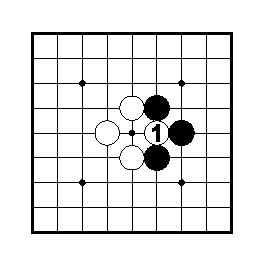
\includegraphics[width=.9\textwidth]{3 - Dia 26}
      \caption*{\emph{Dia.\@~26. Branco captura}}
  \end{subfigure}
  \hfill
  \begin{subfigure}[t]{.3\textwidth}
      \centering
        \captionsetup{justification=centering,singlelinecheck=false,margin={.075in,.05in}}
      
\includegraphics[width=.9\textwidth]{3 - Dia 27}
      \caption*{\emph{Dia.\@~27. Resultado}}
  \end{subfigure}
\end{figure}

Na posição do \emph{Dia.\@~25}, suponha que seja o turno branco. Ele pode capturar uma pedra preta jogando em 1 no \emph{Dia.\@~26}. O resultado é mostrado no \emph{Dia.\@~27}.

Se Preto agora captura com 2 no \emph{Dia.\@~28}\ldots

\pagebreak

\begin{figure}[h]
  \centering
  \begin{subfigure}[t]{.3\textwidth}
      \centering
      \captionsetup{justification=raggedright,singlelinecheck=false,margin={.05in,.05in}}
      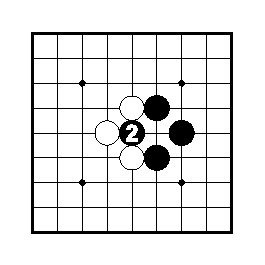
\includegraphics[width=1\textwidth]{3 - Dia 28}
      \caption*{\emph{Dia.\@~28. Uma jogada ilegal}}
  \end{subfigure}
  \hfill
  \begin{subfigure}[t]{.3\textwidth}
      \centering
      \captionsetup{justification=raggedright,singlelinecheck=false,margin={.225in,.05in}}
      
\includegraphics[width=1\textwidth]{3 - Dia 29}
      \caption*{\emph{Dia.\@~29. Mesma posição}}
  \end{subfigure}
  \hfill
  \begin{subfigure}[t]{.3\textwidth}
      \centering
      \captionsetup{justification=raggedright,singlelinecheck=false,margin={.125in,.05in}}
      
\includegraphics[width=1\textwidth]{3 - Dia 30}
      \caption*{\emph{Dia.\@~30. A jogada 3 resolve o ko}}
  \end{subfigure}
\end{figure}

A posição do \emph{Dia.\@~29} é o resultado. Mas, ora, essa é a mesma posição do \emph{Dia.\@~25}. Pela \emph{Regra 7}, isso não é permitido, então Preto precisa jogar em outro lugar. Por exemplo, ele poderia jogar 2 no \emph{Dia.\@~30}. Isso oferece a Branco a oportunidade de conectar em 3, resolvendo o ko.

No \emph{Dia.\@~31}, é o turno Branco a jogar. Uma luta de ko está prestes a acontecer no entorno da pedra preta marcada, que está em atari. O que você acha desta posição? Consegue prever os próximos movimentos? É um grande desafio, tanto em termos de briga de ko como em termos de precisão de jogadas de fim de partida\ldots

\begin{figure}[h]
    \centering
    \captionsetup{justification=centering}
    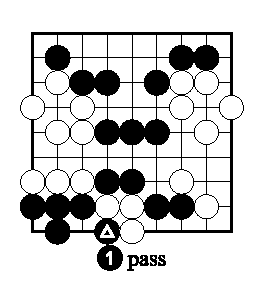
\includegraphics[width=.35\textwidth]{3 - Dia 31}
    \caption*{\emph{Dia.\@~31. Branco a jogar}}
\end{figure}

\pagebreak

Se Branco captura com 1 no \emph{Dia.\@~32}, Preto não pode imediatamente recapturar porque isso reverteria a posição de volta para o \emph{Dia.\@~31}, então ele jogará em outro lugar com Preto 2. Esse tipo de movimento é chamado de \emph{ameaça de ko}.

\begin{figure}[h]
  \centering
  \begin{subfigure}[t]{.3\textwidth}
      \centering
      \captionsetup{justification=raggedright,singlelinecheck=false,margin={.25in,.05in}}
      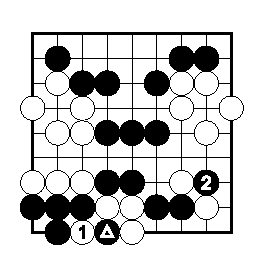
\includegraphics[width=1\textwidth]{3 - Dia 32}
      \caption*{\emph{Dia.\@~32. Uma ameaça de ko}}
  \end{subfigure}
  \hfill
  \begin{subfigure}[t]{.3\textwidth}
      \centering
      \captionsetup{justification=raggedright,singlelinecheck=false,margin={.20in,.05in}}
      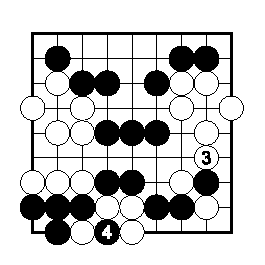
\includegraphics[width=1\textwidth]{3 - Dia 33}
      \caption*{\emph{Dia.\@~33. Branco captura}}
  \end{subfigure}
  \hfill
  \begin{subfigure}[t]{.3\textwidth}
      \centering
      \captionsetup{justification=raggedright,singlelinecheck=false,margin={.05in,.05in}}
      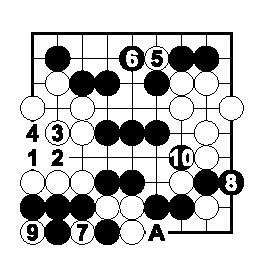
\includegraphics[width=1\textwidth]{3 - Dia 34}
      \caption*{\emph{Dia.\@~34. Resolvendo o ko}}
  \end{subfigure}
\end{figure}

Se Branco responde a essa ameaça com 3 no \emph{Dia.\@~33}, Preto pode recapturar com 4, pois a troca de Preto 2--Branco 3 faz com que a posição global do tabuleiro seja diferente do \emph{Dia.\@~31}. É agora a vez do Branco de encontrar uma ameaça de ko.

Branco corta com 5 no \emph{Dia.\@~34}. Preto poderia ignorar Branco 5 e capturar três pedras em \textbf{A}, e assim  resolver o ko, mas suponhamos que ele responda Branco 5 com 6. Branco pode agora recapturar o ko com 7. Preto precisa fazer outra ameaça de ko com 8. Talvez Branco ignorará essa ameaça e capturará quatro pedras com 9, finalizando a briga pelo ko. Preto obtém alguma compensação com 10.